\documentclass[10pt]{../formats/RU}
%%%% delimiters
\DeclarePairedDelimiter\parens{\lparen}{\rparen}
\DeclarePairedDelimiter\bracks{\lbrack}{\rbrack}
\DeclarePairedDelimiter\braces{\lbrace}{\rbrace}
\DeclarePairedDelimiter\abs{\lvert}{\rvert}
\DeclarePairedDelimiter\norm{\lVert}{\rVert}
\DeclarePairedDelimiter\angles{\langle}{\rangle}
\DeclarePairedDelimiter\ceil{\lceil}{\rceil}
\DeclarePairedDelimiter\floor{\lfloor}{\rfloor}

%%%% math operators naming
\DeclareMathOperator*{\argmax}{\textnormal{argmax}}
\DeclareMathOperator*{\argmin}{\textnormal{argmin}}
\DeclareMathOperator{\tr}{\textnormal{tr}}
\DeclareMathOperator{\eig}{\textnormal{eig}}
\DeclareMathOperator{\sgn}{\textnormal{sgn}}
% \let\det\relax % "Undefine" \det
% \DeclareMathOperator{\det}{\textnormal{det}} % already defined in mathtools
\DeclareMathOperator{\diag}{\textnormal{diag}}
\DeclareMathOperator{\rank}{\textnormal{rank}}
\DeclareMathOperator{\Vol}{\textnormal{Vol}}   % volume
\DeclareMathOperator{\Surf}{\textnormal{Surf}} % surface area

%%%% Transforms! -- requires mathtools package
\newcommand*{\LapTrans}{\xleftrightarrow{\mathcal{Z}}}
\newcommand*{\ZTrans}{\xleftrightarrow{\mathcal{L}}}
\newcommand*{\CTFS}{\xleftrightarrow{\textnormal{CTFS}}}
\newcommand*{\CTFT}{\xleftrightarrow{\textnormal{CTFT}}}
\newcommand*{\DTFS}{\xleftrightarrow{\textnormal{DTFS}}}
\newcommand*{\DTFT}{\xleftrightarrow{\textnormal{DTFT}}}

%%%% vector font
\let\oldvec\vec
\renewcommand*{\vec}[1]{\mathbf{#1}}
% \newcommand*{\trn}{\!^{\!\intercal}}
\newcommand*{\trn}{\!^{\mathsf{T}}}
% \newcommand*{\coj}{\!^{\dag}} % Text Mode Symbol, Should not be used
% \newcommand*{\coj}{\!^{\dagger}}
\newcommand*{\coj}{\!^{\mathsf{H}}}
\newcommand*{\inv}{^{-1}}

%%%% number systems
\DeclareMathOperator{\R}{\mathbb{R}}
\DeclareMathOperator{\C}{\mathbb{C}}
\DeclareMathOperator{\N}{\mathbb{N}}
\DeclareMathOperator{\Z}{\mathbb{Z}}
\DeclareMathOperator{\F}{\mathbb{F}}
\DeclareMathOperator{\Q}{\mathbb{Q}}

%%%% STATISTICS AND PROBABILITY
\newcommand*{\Var}{\mathop{\textnormal{Var}}}
\newcommand*{\Cov}{\mathop{\textnormal{Cov}}}
\newcommand*{\Corr}{\mathop{\textnormal{Corr}}}
\newcommand*{\MSE}{\mathop{\textnormal{MSE}}}
\newcommand*{\MSD}{\mathop{\textnormal{MSD}}}
\newcommand*{\NSD}{\mathop{\textnormal{NSD}}}

\newcommand*{\E}[1]{\mathbb{E}\bracks*{#1}}
\newcommand*{\condE}[2]{\mathbb{E}\bracks*{#1 \mid #2}}
\renewcommand*{\P}[1]{\mathbb{P}\parens*{#1}}
\newcommand*{\condP}[2]{\mathbb{P}\parens*{#1 \mid #2}}

\DeclareMathOperator{\Bern}{\mathsf{Bern}}
\DeclareMathOperator{\Unif}{\mathsf{Unif}}
\DeclareMathOperator{\Expv}{\mathsf{Exp}}
\DeclareMathOperator{\Poi}{\mathsf{Poi}}
\DeclareMathOperator{\Gamv}{\mathsf{Gamma}}
\DeclareMathOperator{\Dirv}{\mathsf{Dir}}
\DeclareMathOperator{\Mult}{\mathsf{Mult}}
\DeclareMathOperator{\Beta}{\mathsf{Beta}}
\DeclareMathOperator{\Geomv}{\mathsf{Geom}}
\DeclareMathOperator{\Binomv}{\mathsf{Binom}}
\DeclareMathOperator{\NegBinomv}{\mathsf{NB}}
\DeclareMathOperator{\Lap}{\mathsf{Lap}}
\DeclareMathOperator{\Gaus}{\mathsf{N}}
\DeclareMathOperator{\Weibull}{\mathsf{Weibull}}


\DeclareMathOperator{\iidsim}{\stackrel{\textnormal{i.i.d.}}{\sim}}
\DeclareMathOperator{\diff}{\mathop{}\!\textnormal{d}}

%%%% Special norms and linear algebra stuff
\newcommand*{\subgnorm}[1]{\norm*{#1}_{\psi_2}}
\newcommand*{\subexpnorm}[1]{\norm*{#1}_{\psi_1}}
\newcommand*{\frobnorm}[1]{\norm*{#1}_{\textnormal{F}}}
\newcommand*{\opnorm}[1]{\norm*{#1}_{\textnormal{op}}}
\newcommand*{\Lipnorm}[1]{\norm*{#1}_{\textnormal{Lip}}}

%%%%
\newcommand*{\set}[1]{\braces*{\,#1\,}}
\newcommand*{\ie}{\textnormal{i.e.\ }}
\newcommand*{\eg}{\textnormal{e.g.\ }}
\newcommand*{\etc}{\textnormal{etc.\ }}
\newcommand*{\iid}{\textnormal{i.i.d.\ }}

%Theorem style
\declaretheorem[numbered=no, style=definition]{axiom}
\declaretheorem[numberwithin=section,style=definition]{definition}
\declaretheorem[sibling=definition]{theorem, lemma, corollary, proposition, conjecture}
\declaretheorem[numbered=no,style=remark]{remark, claim}

%Information to be included in the title page:
\title[Random Fourier Feature]{Random Features for Large-Scale Kernel Machines~\footcite{NIPS2007_013a006f}
}
\author[Kai] % (optional, for multiple authors)
{Kailong Wang\inst{1}
%\and Someone Else\inst{2}
}
\institute[Rutgers] % (optional)
{
  \inst{1}%
  % Ph.D.\ of ECE\\
  Rutgers University
  % \and
  % \inst{2}%
  % Faculty of Statistics\\
  % Very Famous University
}
\date[\today] % (optional)
{
  % ECE 539 HDP,
  \today}

 \addbibresource{bib.bib}


\begin{document}
\frame{\titlepage}
%---------------------------------------------------------
%This block of code is for the table of contents after
%the title page
\begin{frame}
\frametitle{Table of Contents}
\tableofcontents
\end{frame}
%---------------------------------------------------------



\section{Motivation}
%---------------------------------------------------------
\begin{frame}
  \frametitle{Linear Non-separable Problem}
  Consider a binary classification problem with non-linear samples.
  \begin{figure}
    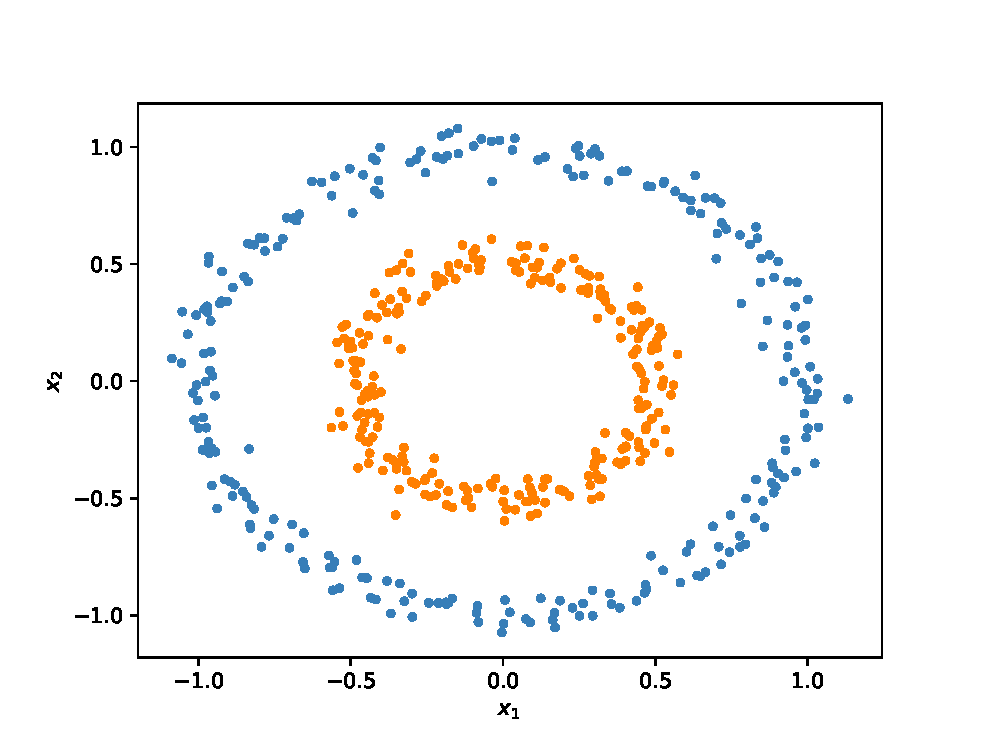
\includegraphics[height=0.5\textheight]{./figs/2d_poly_circle.eps}%
  \end{figure}
  \eg For the above dataset $\mtx{X}=[\vec{x}_1, \vec{x}_2, \ldots, \vec{x}_N]$ where $\vec{x}_i\in \R^2$, a linear decision boundary does not exist.
\end{frame}
%---------------------------------------------------------
\begin{frame}
  \frametitle{Lifting}
  One idea is \textbf{LIFTING} the samples into a high dimensional space in which the samples are linearly separable.
  \begin{figure}
    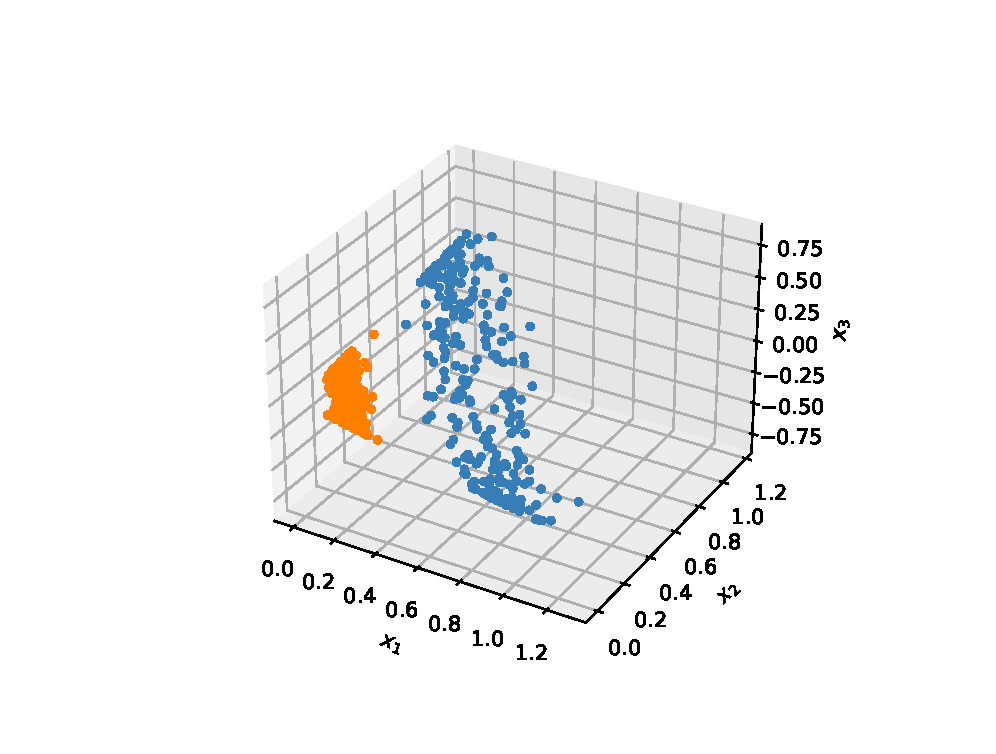
\includegraphics[height=0.45\textheight]{./figs/3d_poly_circle.eps}%
  \end{figure}
  In this case, the function
  $
  \phi(\mathbf{x}_i) = \bracks*{x_{i,1}^2 , x_{i,2}^2 , \sqrt{2}x_{i,1}x_{i,2}},
  $
  lifts the samples into $\R^3$ and the samples are linearly separable.
\end{frame}
%---------------------------------------------------------
\begin{frame}
  \frametitle{SVM~\footcite{boyd2004convex}}
  The idea of lifting has been implemented in many classification algorithms such as \emph{support vector machine} (SVM).
  \begin{itemize}
    \item Dual Problem of SVM{
      \begin{align*}
        \max_{\vec{\alpha}} &\sum_{n=1}^N\alpha_n - \frac{1}{2}\sum_{n=1}^{N}\sum_{m=1}^{N}\alpha_n\alpha_m y_ny_m\angles*{\mathbf{x}_n, \mathbf{x}_m}
      \end{align*}
    }
    \item Dual Problem with Lifting {
      \begin{align*}
        \max_{\vec{\alpha}} &\sum_{n=1}^N\alpha_n - \frac{1}{2}\sum_{n=1}^{N}\sum_{m=1}^{N}\alpha_n\alpha_m y_ny_m\angles*{\phi(\mathbf{x}_n), \phi(\mathbf{x}_m)}
      \end{align*}
    }
  \end{itemize}
  This is the hard-margin SVM. The soft-margin SVM is similar.
\end{frame}
%---------------------------------------------------------
\begin{frame}
\frametitle{Curse of Dimensionality--Type I}
  \begin{align*}
    \angles*{\phi(\mathbf{x}_n), \phi(\mathbf{x}_m)}
    &= \bracks*{x_{n,1}^2 , x_{n,2}^2 , \sqrt{2}x_{n,1}x_{n,2}}\trn\bracks*{x_{m,1}^2 , x_{m,2}^2 , \sqrt{2}x_{m,1}x_{m,2}} \\
    &= x_{n,1}^2x_{m,1}^2 + x_{n,2}^2x_{m,2}^2 + 2x_{n,1}x_{n,2}x_{m,1}x_{m,2}
  \end{align*}
As shown in the given example, the inner product (a constant value) of the lifted vector has computational complexity depends on lifted dimension. For a function lifts the original vector space to a much higher dimension, such a calculation can be computationally thirsty. Alternatively, this can be done as follows, whose computational complexity only depends on the dimension of the original vector space.
  \begin{align*}
    (\angles*{\mathbf{x}_n, \mathbf{x}_m})^2
    &= \parens*{\bracks*{x_{n,1} , x_{n,2}}\trn\bracks*{x_{m,1} , x_{m,2}}}^2 \\
    &= \parens*{x_{n,1}x_{m,1} + x_{n,2}x_{m,2}}^2 \\
    &= x_{n,1}^2x_{m,1}^2 + x_{n,2}^2x_{m,2}^2 + 2x_{n,1}x_{n,2}x_{m,1}x_{m,2} \\
    &= \angles*{\phi(\mathbf{x}_n), \phi(\mathbf{x}_m)}
  \end{align*}
\end{frame}
%---------------------------------------------------------
\begin{frame}
  \frametitle{Kernel Trick}
  The type of function, such as $(\angles*{\cdot, \cdot})^2$, that provides a computationally efficient way to compute the inner product in the high dimensional space is called a \textbf{Kernel Function}.
  \[
    K(\cdot,\cdot) = \angles*{\phi(\cdot),\phi(\cdot)}
  \]
  The matrix that is formed by stacking the kernel function for all samples is called the \textbf{Kernel Matrix} $\mathbf{K}$, which is a \textbf{Gram Matrix},
  \[
    \mathbf{K}_{nm} \equiv K(\mathbf{x}_n, \mathbf{x}_m).
  \]
  Some kernel functions can lift the original vector space to an infinite dimensional space.
  The algorithms involve kernel trick is called \textbf{Kernel Machines}.
\end{frame}
%---------------------------------------------------------
\begin{frame}
  \frametitle{Curse of Dimensionality--Type II}
  Another famous kernel machine is kernel ridge regression (KRR). With $\vec{y}\in R^N$, $\mtx{X}\in\R^{N\times d}$, and $\phi_{d\rightarrow k}(\cdot):\R^d\rightarrow\R^k$,
  % the loss function is
  %     \begin{align*}
  %       \mathcal{L}(\vec{w})=\argmin_{\vec{w}}(\vec{y}-\phi(\mtx{X})\vec{w})\trn(\vec{y}-\phi(\mtx{X})\vec{w}) + \lambda\vec{w}\trn\vec{w}.
  %     \end{align*}
  the normal equation of KRR is (using matrix inversion lemma)
  \begin{align}
    \vec{w} &= (\phi(\mtx{X})\trn\phi(\mtx{X})+\lambda\mathbf{I}_k)^{-1}\phi(\mtx{X})\trn\vec{y} \label{illproblem} \\
    &= \phi(\mtx{X})\trn(\lambda\mtx{I}_N+\phi(\mtx{X})\phi(\mtx{X})\trn)^{-1}\vec{y} \label{inversion}\\
    &= \phi(\mtx{X})\trn(\lambda\mtx{I}_N+\mathbf{K})^{-1}\vec{y}.
  \end{align}
  For any input $\vec{x^*}$, the prediction is (let $\vec{\alpha}=(\lambda\mtx{I}_N+\mathbf{K})^{-1}\vec{y}$)
  \begin{align}
    \phi(\vec{x^*})\trn\vec{w}
    &= \sum_{i=1}^{N}K(\phi(\vec{x^*}), \phi(\vec{x}_i))\vec{\alpha}_i.
  \end{align}
  Eq.~\eqref{illproblem} is problematic since $k\rightarrow\infty$. Common approach solves eq.~\eqref{inversion} with $O(N^3)$ time and $O(N^2)$ memory. This is not scalable in modern big data era, where $N\rightarrow\infty$.
  % Computing $\mathbf{K}$ requires $O(N^2d)$ time. Inference with $\mathbf{K}$ requires $O(Nd)$ time.
\end{frame}
%---------------------------------------------------------
\begin{frame}
  \frametitle{Motivation}
  Can we find a \textbf{Kernel Function} $K(\cdot, \cdot)$, which is equivalent to lifting $\mathbf{X}$ to $\R^s$ with $d < s\ll k$, while not sacrifices model performance?

  In such a case, we can solve eq.~\eqref{illproblem} instead of eq.~\eqref{inversion}, where the algorithm complexity dependents on $s$, where $s\ll N$.
  % which only needs $s$ samples with $s\ll N$
\end{frame}
%---------------------------------------------------------


\section{Random Fourier Features (RFF)}
%---------------------------------------------------------
\begin{frame}
\frametitle{Some Prerequisites}
\begin{block}{Definition: Shift Invariant Kernel (Radial Basis Function (RBF))}
  A kernel function $K(\vec{x}_n, \vec{x}_m)$ is called \textbf{shift invariant} if it can be written as $K(\vec{x}_n, \vec{x}_m) = k(\vec{x}_n-\vec{x}_m)$ for some function $k(\cdot)$

  (\eg $K_{Gaussian}(\vec{x}_n,\vec{x}_m)=\exp(-\gamma\norm{\vec{x}_n-\vec{x}_m}_2^2)$).
\end{block}
\begin{alertblock}{Mercer’s Theorem}
  A continuous function $K(\vec{x}_n, \vec{x}_m)$ is a valid kernel function if and only if the kernel matrix $\mathbf{K}$ is \textbf{positive semi-definite}.
\end{alertblock}
\begin{alertblock}{Bochner's Theorem}
  A continuous function $k(\cdot)$ is \textbf{positive semi-definite} if and only if it is the Fourier transform of a non-negative measure.
\end{alertblock}
\end{frame}
%---------------------------------------------------------
\begin{frame}
  \frametitle{Random Fourier Features}
  \begin{exampleblock}{Conclusion}
    A continuous \textbf{shift invariant} kernel $K(\vec{x}_n, \vec{x}_m)$, which is \textbf{positive semi-definite} (Mercer's Theorem), is the Fourier transform of a non-negative measure $p(\cdot)$.
    \begin{align}
      \phi(\vec{x}_n)\trn\phi(\vec{x}_m)
      &= K(\vec{x}_n, \vec{x}_m) = k(\vec{x}_n-\vec{x}_m) \\
      &=\int_{\R^d}p(\vec{\omega})\exp(i\vec{\omega}\trn(\vec{x}_n-\vec{x}_m))\diff\vec{\omega} \\
      &= \mathbb{E}_{\vec{\omega}}\bracks*{\xi_{\vec{\omega}}(\vec{x}_n)\coj\xi_{\vec{\omega}}(\vec{x}_m)}\label{rffinC}
    \end{align}
    Here
    $
    \xi_{\vec{\omega}}(\vec{x}_i)=\exp(i\vec{\omega}\trn(\vec{x}_i))
    $.
  \end{exampleblock}
\end{frame}
%---------------------------------------------------------
\begin{frame}
  \frametitle{Random Fourier Features}
  Since both the $p(\cdot)$ and $k(\triangle)$ are real-valued, we can replace $\xi_{\vec{\omega}}(\vec{x}_i)=\exp(i\vec{\omega}\trn(\vec{x}_i))$ with
  $
  z_{\vec{\omega}}(\vec{x}_i)=\sqrt{2}\cos(\vec{\omega}\trn(\vec{x}_i)+b)$. Then eq.~\eqref{rffinC} becomes $\mathbb{E}_{\vec{\omega}}[z_{\vec{\omega}}(\vec{x}_n)\trn z_{\vec{\omega}}(\vec{x}_m)]$, which means $z_{\vec{\omega}}(\vec{x}_n)\trn z_{\vec{\omega}}(\vec{x}_m)$ is an unbiased estimator of $\phi(\vec{x}_n)\trn\phi(\vec{x}_m)$.

  Let $\vec{\omega}$ been drawn from $p(\vec{\omega})$ and $b$ been uniformly drawn from $[0, 2\pi]$, the calculation of $\phi(\vec{x}_n)\trn\phi(\vec{x}_m)$ becomes a sampling problem.

  To further reduce the variance of the estimator, we can randomly draw $s$ samples of $\vec{\omega}$ and $b$, normalize each corresponding $z_{\vec{\omega}}(\vec{x}_i)$ by $\sqrt{s}$, and concatenate them into one vector. Then the inner product $z(\vec{x}_n)\trn z(\vec{x}_m)=\frac{1}{s}\sum_{j=1}^{s}z_{\vec{\omega}_j}(\vec{x}_n)\trn z_{\vec{\omega}_j}(\vec{x}_m)$
  % \item <4-> \textbf{Question:} The author samples $\vec{\omega}$ from $\R^d$ and average over $s$ samples in the following algorithm. However, $d\&s$ seems can be arbitrary number based on the above derivation.
\end{frame}
%---------------------------------------------------------
\begin{frame}
  \frametitle{Algorithm}
  \begin{algorithm}[H]
    \caption{Random Fourier Features}\label{RFF}
    \begin{algorithmic}
    \Require A shift invariant kernel $K(\vec{x}_n, \vec{x}_m) = k(\vec{x}_n- \vec{x}_m)=k(\triangle)$.
    \Ensure A randomized feature map $z(\cdot): \R^d\rightarrow\R^s$ so that $z(\vec{x}_n)\trn z(\vec{x}_m)\approx K(\vec{x}_n, \vec{x}_m)$.
    \State Compute the Fourier transform $p(\cdot)$ of the kernel $K: p(\vec{\omega})=\frac{1}{2\pi}\int \exp(-i\vec{\omega}\trn\triangle)k(\triangle)\diff\triangle$
    \State Draw $s$ \iid samples $\vec{\omega}_1, \vec{\omega}_2, \ldots, \vec{\omega}_s \in \R^d$ from $p(\vec{\omega})$ and $s$ \iid samples $b_1, b_2, \ldots, b_s \in [0, 2\pi]$.
    \State Let $z(\vec{x}_i)\equiv \sqrt{\frac{2}{s}}[\cos(\vec{\omega}_1\trn\vec{x}_i+b_1), \cos(\vec{\omega}_2\trn\vec{x}_i+b_2), \ldots, \cos(\vec{\omega}_s\trn\vec{x}_i+b_s)]$
    \end{algorithmic}
  \end{algorithm}
\end{frame}
%---------------------------------------------------------
\begin{frame}{Common RFF}
  \centering
  \begin{tabular}{c c c}
    Kernel & $K(\triangle)$ & $p(\vec{\omega})$ \\
    \hline
    Gaussian & $\exp(-\gamma\norm{\triangle}_2^2)$ & $(2\pi)^{-\frac{s}{2}}\exp{-\gamma\norm{\vec{\omega}}_2^2}$\\
    Laplacian & $\exp(-\norm{\triangle}_1)$ & $\prod\limits_{d}(\pi(1+\omega_d^2))^{-1}$\\
    Cauchy & $\prod\limits_{d}2(1+\triangle_d^2)^{-1}$ & $\exp(-\norm{\vec{\omega}}_1)$
  \end{tabular}
\end{frame}
%---------------------------------------------------------


\section{Convergence of RFF}
%---------------------------------------------------------
\begin{frame}
  \frametitle{Convergence with Hoeffding's Inequality~\footcite{vershynin_hdp}}
  \begin{alertblock}{Theorem: Hoeffding's Inequality}
    Let $X_1, X_2,\cdots, X_N$ be independent random variables. Assume that $X_i \in [m_i, M_i]$ for every $i$. Then, for any $\epsilon > 0$, we have
    \[
    \P{\abs*{\sum_{i=i}^{N}(X_i-\E{X_i})}\geq \epsilon} \leq 2\exp\parens*{-\frac{2\epsilon^2}{\sum_{i=1}^{N}(M_i-m_i)^2}}.
    \]
  \end{alertblock}
  \begin{exampleblock}{Bound for \emph{any} pair of samples $\vec{x}_n$ and $\vec{x}_m$}
    Given $z_{\vec{\omega}}$ is bounded random variable between $[-\sqrt{2/s}, \sqrt{2/s}]$, with Hoeffding's Inequality, we have
    \begin{align*}
      \P{\abs{z(\vec{x}_n)\trn z(\vec{x}_m)-K(\vec{x}_n, \vec{x}_m)}\geq \epsilon} \leq 2\exp\parens*{-\frac{s\epsilon^2}{4}}.
    \end{align*}
  \end{exampleblock}
\end{frame}
%---------------------------------------------------------
\begin{frame}
  \frametitle{Convergence}
  \begin{exampleblock}{Bound for the \textbf{Kernel Matrix}}
    Let $\mathcal{M}$ be a compact subset of $\R^d$ with diameter $\textnormal{diam}(\mathcal{M})$. Then, for the mapping $z$ defined in Algorithm~\ref{RFF}, we have
    \begin{align*}
      \P{\sup_{x,y\in\mathcal{M}}\abs{z(\vec{x}_n)\trn z(\vec{x}_m)-K(\vec{x}_n, \vec{x}_m)}\geq \epsilon} \\
      \leq 2^8\parens*{\frac{\sigma_{p(\cdot)}\textnormal{diam}(\mathcal{M})}{\epsilon}}^2\exp\parens*{-\frac{s\epsilon^2}{4(d+2)}}.
    \end{align*}
    The $\sigma_{p(\cdot)}^2=\mathbb{E}_{p(\cdot)}\bracks*{\vec{\omega}\trn\vec{\omega}}$ is the second moment of the Fourier transform of the $K(\cdot,\cdot)$.
  \end{exampleblock}
  The proof of this bound uses the knowledge of $\epsilon$-net and $\epsilon$-covering number.
\end{frame}
%---------------------------------------------------------
\begin{frame}
  \frametitle{Experiment}
  \begin{table}[]
    \centering
    \begin{tabular}{|l|l|l|}
    \hline
    \textbf{Datasets} &
      \textbf{Fourier + LS} &
      \textbf{SVM} \\ \hline
    \begin{tabular}[c]{@{}l@{}}CPU\\ regression\\ 6,500 instances; 21 dims\end{tabular} &
      \begin{tabular}[c]{@{}l@{}}3.6\%\\ 20 secs\\ s = 300\end{tabular} &
      \begin{tabular}[b]{@{}l@{}}5.5\%\\ 51 secs\end{tabular} \\ \hline
    \begin{tabular}[c]{@{}l@{}}Census\\ regression\\ 18,000 instances; 119 dims\end{tabular} &
      \begin{tabular}[c]{@{}l@{}}5\%\\ 36 secs\\ s = 500\end{tabular} &
      \begin{tabular}[b]{@{}l@{}}8.8\%\\ 7.5 mins\end{tabular} \\ \hline
    \begin{tabular}[c]{@{}l@{}}Adult\\ classification\\ 32,000 instances; 123 dims\end{tabular} &
      \begin{tabular}[c]{@{}l@{}}14.9\%\\ 9 secs\\ s = 500\end{tabular} &
      \begin{tabular}[b]{@{}l@{}}14.8\%\\ 73 mins\end{tabular} \\ \hline
    \begin{tabular}[c]{@{}l@{}}KDDCUP99\\ classification\\ 4,900,000 instances; 127 dims\end{tabular} &
      \begin{tabular}[c]{@{}l@{}}7.3\%\\ 1.5 mins\\ s = 50\end{tabular} &
      \begin{tabular}[b]{@{}l@{}}6.2\% (18\%)\\ 1.4 secs (20 secs)\end{tabular} \\ \hline
    \end{tabular}
    \caption{Comparison of testing error and training time between ridge regression with random features and Support Vector Machine. For classification tasks, the percent of testing points incorrectly predicted is reported. For regression tasks, the RMS error normalized
    by the norm of the ground truth is reported. }
    \label{tab:my-table}
    \end{table}
\end{frame}
%---------------------------------------------------------

\end{document}